\documentclass[11pt,a4paper]{report}

\usepackage{amssymb,amsmath,epsfig,float,subfig,hyperref,multicol}

\usepackage{xcolor}

\definecolor{SCSUred}{HTML}{CD1041}

\hypersetup{colorlinks=true,linkcolor=SCSUred,urlcolor=SCSUred}

\usepackage{enumerate}
\usepackage{tikz}
\usetikzlibrary{arrows}
\usetikzlibrary{patterns}
\usetikzlibrary{decorations}
%%\usetikzlibrary{intersections}
\usetikzlibrary{matrix}
\usetikzlibrary{snakes}
\usetikzlibrary{calc}
\usetikzlibrary{backgrounds}

\definecolor{linecolor}{HTML}{0074C8}
\definecolor{linecolor2}{HTML}{C80200}

\newcommand{\imagebullet}[1]{\includegraphics[width=0.5cm]{#1}}


\pagestyle{empty}
\setlength{\textwidth}{7in}
\setlength{\textheight}{10in}
\setlength{\oddsidemargin}{-25pt}
\setlength{\evensidemargin}{-25pt}
\setlength{\topmargin}{-50pt}

\usepackage[english]{babel}
\usepackage[utf8]{inputenc}
\usepackage{fancyhdr}
 
%%\pagestyle{fancy}
\renewcommand{\headrulewidth}{0pt}
%%\fancyhf{}
%%\rhead{Share\LaTeX}
%%\lhead{Guides and tutorials}
%%\cfoot{OVER}

\newcommand{\DueA}{Tuesday, October 22}
\newcommand{\DueB}{Thursday, October 24}
\newcommand{\DueC}{Thursday, October 31}

\begin{document}

\begin{figure}[ht]
\begin{flushright}
	\includegraphics[width=2.0in]{U_PriHorz_WhtLtBG.jpg}
	\end{flushright}
\end{figure}

\vspace{-12mm}

\begin{flushleft}
\Large\bf \href{https://activecalculus.org/single/sec-3-1-tests.html}{3.1 - Using Derivatives to Identify Extreme Values}\rm
%%Daily Preparation - \DueA \rm
\end{flushleft}


\vspace{8pt}

\noindent {\Large\bf{Overview}} \\
In our next meeting, we start Chapter 3: Using Derivatives. The theme of this chapter centers on what we can learn from key information regarding the derivative of a function. In the first section, Section 3.1, we focus on how the derivative detects extreme values of functions. That is, we investigate how information from the derivative function can tell us whether the original function has a relative maximum or relative minimum at a given point. While many of the ideas in this section will be natural and intuitive (and ones we've discussed briefly to some extent earlier in the course), there is considerable new language and reasoning to learn and understand.



\vspace{16pt}

\noindent {\Large\bf{To prepare for class}} \\
Complete all actions listed below.  Respond to the questions highlighted with {\color{SCSUred}{\boxed{Submit}}}.  %% by the start of class on {\bf{\DueA}}.  A single .pdf should be uploaded to D2L Brightspace.
\begin{itemize} \itemsep -2pt % Reduce space between items

\item {\bf{Read}} motivating questions and the introduction to \href{https://activecalculus.org/single/sec-3-1-tests.html}{section 3.1} (up until Preview Activity 3.1.1).

\item[{\color{SCSUred} \boxed{Submit}}]  {\bf{Do}} \href{https://activecalculus.org/single/sec-3-1-tests.html#svs}{Preview Activity 3.1.1}.

\item {\bf{Do}} these problems.
\begin{enumerate}
\item Plot the graph of $f(x) = \sqrt{|x|}$ on each of the following domains.  Then, determine if the function has a global maximum and a global minimum on that domain.  Feel free to use \href{https://www.geogebra.org/classic}{GeoGebra} to verify your thinking.  
\begin{enumerate}
\item $[-4,4]$
\vspace{10mm}
\item $[-4,0)$
\vspace{10mm}
\item $(-4,0)$
\vspace{10mm}
\item $(-\infty, \infty)$
\end{enumerate}


\vspace{-55mm}
 \begin{figure}[H]
\flushright
{
  \begin{tikzpicture}[thick,scale=1.25] [domain=-4:4]
\draw[step=1cm,color=gray!50] (-4,-1) grid (4,3);
   \draw [black!80,line width=0.3pt,-latex] (0,0) -- (4,0) node [below] at (3.75,0) {$x$};
   \draw [black!80,line width=0.3pt,-latex] (0,0) -- (-4,0);
   \draw [black!80,line width=0.3pt,-latex] (0,0) -- (0,3) node [right] at (0,2.75) {$y$};
   \draw [black!80,line width=0.3pt,-latex] (0,0) -- (0,-1);
  
\foreach \x/\xtext in {-3/-3, -2/-2,-1/-1, 1/1, 2/2}
    \draw[shift={(\x,0)}] (0pt,3pt) -- (0pt,-3pt) node[below] {$\xtext$};
\foreach \y/\ytext in { 1/1, 2/2}
    \draw[shift={(0,\y)}] (-2pt,0pt) -- (2pt,0pt) node[left] {$\ytext$};
\end{tikzpicture}}  
\end{figure}
\vspace{5mm}

\item Even a closed, bounded interval does not guarantee the existence of global extrema.  For example, on $[0,3]$ plot the graph of $$f(x) = \left\{ \begin{array}{cc} x+1 & {\rm{if \ }} 0 \leq x <1 \\ -x & {\rm{if \ }} 1 \leq x <2 \\ 0 & {\rm{if \ }} 2 \leq x \leq 3 \end{array} \right\}.$$
\vspace{-20mm}
 \begin{figure}[H]
\flushright
{
  \begin{tikzpicture}[thick,scale=1] [domain=-4:4]
\draw[step=1cm,color=gray!50] (-1,-3) grid (4,3);
   \draw [black!80,line width=0.3pt,-latex] (0,0) -- (4,0) node [below] at (3.75,0) {$x$};
   \draw [black!80,line width=0.3pt,-latex] (0,0) -- (-1,0);
   \draw [black!80,line width=0.3pt,-latex] (0,0) -- (0,3) node [right] at (0,2.75) {$y$};
   \draw [black!80,line width=0.3pt,-latex] (0,0) -- (0,-3);
\foreach \x/\xtext in {-1/-1, 1/1, 2/2, 3/3}
    \draw[shift={(\x,0)}] (0pt,3pt) -- (0pt,-3pt) node[below] {$\xtext$};
\foreach \y/\ytext in {-2/-2, -1/-1, 1/1, 2/2, 3/3}
    \draw[shift={(0,\y)}] (-2pt,0pt) -- (2pt,0pt) node[left] {$\ytext$};
\end{tikzpicture}}  
\end{figure}
\end{enumerate}

\item {\bf{Watch}} video \href{https://www.youtube.com/watch?v=tvF3Rq0urvI&feature=emb_title}{Finding Local and Global Extrema (5:05)}. 

\item[\imagebullet{CopilotLogo.jpg}] Ask {\bf{Copilot}} ``In calculus, why are critical numbers named the way that they are?"

\item {\bf{Read}} \href{https://activecalculus.org/single/sec-3-1-tests.html#aiK}{section 3.1.1} (up to Activity 3.1.2).



\item {\bf{Do}} this problem.
\begin{enumerate}
\setcounter{enumi}{2}
\item The graph of a continuous function $f$ is given.  Estimate the location of all relative and global maxima and minima on the domain $[0,10]$.  What do you notice about the derivative of $f$ at these locations?  

 \begin{figure}[H]
\flushright
{
  \begin{tikzpicture}[thick,scale=0.75] [domain=-3:3]
\draw[step=1cm,color=gray!50] (0,0) grid (10,7);
   \draw [black!80,line width=0.3pt,-latex] (0,0) -- (11,0) node [below] at (10.5,0) {$x$};
   %%\draw [black!80,line width=0.3pt,-latex] (0,0) -- (-4,0);
   \draw [black!80,line width=0.3pt,-latex] (0,0) -- (0,7) node [right] at (0,6.5) {$y$};
   %%\draw [black!80,line width=0.3pt,-latex] (0,0) -- (0,-4);
\draw[color=blue, line width=1pt,domain=0:8,smooth]   plot (\x,{0.025*\x*\x*\x*\x-0.433*\x*\x*\x+2.5*\x*\x-5.6*\x+6});
\draw[color=blue, line width=1pt,domain=8:9,smooth] plot(\x,{1.904+2.464*(\x-8)});
\draw[color=blue, line width=1pt,domain=9:10,smooth] plot(\x,{4.368-2.464*(\x-9)});
%%  node[above] at (2,1) {$f(3,y)$};
\foreach \x/\xtext in {2/2, 4/4, 6/6, 8/8, 10/10}
    \draw[shift={(\x,0)}] (0pt,3pt) -- (0pt,-3pt) node[below] {$\xtext$};
\foreach \y/\ytext in {2/2, 4/4, 6/6}
    \draw[shift={(0,\y)}] (-2pt,0pt) -- (2pt,0pt) node[left] {$\ytext$};
\end{tikzpicture}}  
\end{figure}
\end{enumerate}

\item {\bf{Watch}} video \href{https://www.youtube.com/watch?v=7RcLQZdB0LM&feature=emb_title}{Identifying Critical Values Graphically (4:20)}.



\item {\bf{Watch}} video \href{https://www.youtube.com/watch?v=x-efl3Br11E&feature=emb_title}{Finding Critical Values (3:11)}.  

\item[{\color{SCSUred} \boxed{Submit}}]  {\bf{Explore}} applet \href{https://www.geogebra.org/m/EPnuRjtr}{Critical Values}.  Then determine the critical values for the given function in the applet.  What is the behavior of $f'(x)$ on the left and the right of these critical values?  Does that behavior tell you if the critical value is a local maximum or local minimum?  Explain.  

\item {\bf{Do}} the following problem.
\begin{enumerate}
\setcounter{enumi}{3}
\item Consider $f(x)=x^3$.  Locate a critical value of $f$ both graphically and algebraically. Explain why there is no maximum or minimum there. 

 \begin{figure}[H]
\centering
{
  \begin{tikzpicture}[thick,scale=1.75] [domain=-3:3]
%%\draw[step=1cm,color=black!75,dotted] (-1,1) grid (1,1);
   \draw [black!80,line width=0.3pt,-latex] (0,0) -- (1.5,0) node [below] at (1.25,0) {$x$};
   \draw [black!80,line width=0.3pt,-latex] (0,0) -- (-1,0);
   \draw [black!80,line width=0.3pt,-latex] (0,0) -- (0,1.5) node [right] at (0,1.25) {$y$};
   \draw [black!80,line width=0.3pt,-latex] (0,0) -- (0,-1);
\draw[color=blue, line width=1pt,domain=-1:1,smooth]   plot (\x,{\x*\x*\x}) node[above] at (0.5,0.5) {$f$};
\foreach \x/\xtext in {-1/-1, 1/1}
    \draw[shift={(\x,0)}] (0pt,3pt) -- (0pt,-3pt) node[below] {$\xtext$};
\foreach \y/\ytext in {-1/-1, 1/1}
    \draw[shift={(0,\y)}] (-2pt,0pt) -- (2pt,0pt) node[left] {$\ytext$};
\end{tikzpicture}}  
\end{figure}
\end{enumerate}

\item {\bf{Watch}} video \href{https://www.youtube.com/watch?v=9rg5jpFVSFY&feature=emb_title}{Using the First Derivative Test (11:08)}.  This video shows how to apply the First Derivative Test in practice, by using the sign table of the derivative to determine the intervals of increasing/decreasing behavior of a function.



\item[{\color{SCSUred} \boxed{Submit}}] {\bf{Explore}}.   Submit a screenshot with a reasonable score (like Professor Buske got on his first try...see below) to the Activity in the applet: \href{http://webspace.ship.edu/msrenault/GeoGebraCalculus/derivative_app_1_graph_AD.html}{Reconstruct $f$ from its First Derivative}.

\begin{figure}[H]
\begin{center}
	\includegraphics[width=4.75in]{AppletReconstructf.jpg}
	\end{center}
\end{figure}


 

  















\end{itemize}











\vspace{16pt}

\noindent {\Large\bf{After class}}\\
Solidifying the concepts discussed in class through practice is necessary to build your skills. 

%%\noindent {\large\bf{After \DueA}}
\begin{itemize}\itemsep -2pt % Reduce space between items

\item {\bf{Read}} \href{https://activecalculus.org/single/sec-3-1-tests.html#GpT}{section 3.1.2}.

\item {\bf{Watch}} this video \href{https://www.youtube.com/watch?v=2n9PmWWlLeU&feature=emb_title}{The Second Derivative Test (8:58)}. 

\item[\imagebullet{CopilotLogo.jpg}] Ask {\bf{Copilot}} ``In the second derivative test in calculus, what can I conclude when $f''(x) = 0$?"

\item {\bf{Watch}} video \href{https://www.youtube.com/watch?v=Bzj_oXB6yIU&feature=emb_title}{Quick Review - Extreme Values of Functions (4:10)}.   

\item {\bf{Read}} \href{https://activecalculus.org/single/sec-3-1-tests.html#mxc}{section 3.1.3 - Summary}.

%%\item {\bf{Do}} \href{https://activecalculus.org/single/sec-3-1-tests.html#LLc}{Activity 3.1.3}.

\item {\bf{Do}} \href{https://activecalculus.org/single/sec-3-1-tests.html#bkM}{exercises 1-3 in section 3.1.4}.

\item {\bf{Do}} this problem.
\begin{enumerate}
\setcounter{enumi}{5}
%%\item 
%%\begin{enumerate}
%%\item For a positive constant $b$, the surge function $f(t) = te^{-bt}$ gives the quantity of a drug in the body for a time $t \geq 0$.  Find the global maximum and minimum of $f(t)$ on $[0,\infty)$.  
%%\vspace{10mm}
%%\item Find the value of $b$ making $t=10$ the global \\ maximum on $[0, \infty)$.  
%%\vspace{10mm}
%%\end{enumerate}  

%%\vspace{-20mm}
%%\begin{figure}[H]
%%\begin{flushright}
	%%\includegraphics[width=2.75in]{fig_04_23.jpg}
	%%\end{flushright}
%%\end{figure}



\item If $a$ and $b$ are positive constants, find all critical points of $$g(t) = ae^t + be^{-t}.$$  {\it{Hint:}} Try factoring $e^{-t}$ out of the derivative.  





\end{enumerate}

%%\item {\bf{Do}} Activity 2.8.4.   

%%\end{itemize}

%%\noindent {\large\bf{After \DueB}}
%%\begin{itemize}\itemsep -2pt % Reduce space between items 

\item {\bf{Do}} \href{https://activecalculus.org/single/sec-3-1-tests.html#TGn}{exercises 4-7 from section 3.1.4}.

\item {\bf{Start working}} on the \href{https://www.myopenmath.com/index.php}{MOMwork} (MyOpenMath) assignment for this section.  %%This will be due on \DueC. 

\end{itemize}

\pagebreak

\vspace{16pt}

\noindent {\Huge\bf{Extra Prep}}

\vspace{16pt}

\noindent {\Large\bf{Basic learning objectives}}\\
These are the tasks you should be able to perform with reasonable
fluency when you arrive at our next class meeting. Important new
vocabulary words are indicated {\it{in italics}}.  Check each box when you feel confident you have a firm grasp on that objective. 

\begin{itemize} \itemsep -2pt % Reduce space between items
\renewcommand{\labelitemi}{\scriptsize$\square$}
\item Define {\it{local maximum, local minimum, global maximum}}, and {\it{global minimum}}. 
\item Identify the difference between {\it{local}} extrema and {\it{global}} extrema.
\item State the definition of a {\it{critical number}}.

\item Find all critical numbers of a function, given its derivative.

\item State the {\it{First Derivative Test}} and explain both its purpose and how it is used.

\item State and apply the following fact: If the function $f$ has a local extremum at $x=c$, then $c$ is a critical number of $f$.  Be able to give examples demonstrating that the opposite is false: If $c$ is a critical number of $f$, then there is {\it{not}} necessarily a local extremum at $c$.

\item State the {\it{Second Derivative Test}} and explain both its purpose and how it is used.

\item Define {\it{inflection point}}.
\end{itemize}


\vspace{16pt}

\noindent {\Large\bf{Advanced learning objectives}}\\
In addition to mastering the basic objectives, here are the tasks you should be able to perform after class, with practice:
\begin{itemize} \itemsep -2pt % Reduce space between items
\renewcommand{\labelitemi}{\scriptsize$\square$}
\item Construct a sign chart for the first derivative.  Use it to determine the intervals of the increasing/decreasing behavior, as well as the location of extreme values of a function.

\item Construct a sign chart for the second derivative.  Use it to determine the intervals of the concave up/concave down behavior, as well as the location of inflection points of a function.

\item Classify all critical points of a function as local max, min, or neither, using the first or second derivative test.

\item Use a sign chart to determine the intervals on which a function is concave up or concave down and to find inflection points.

\item Use sign charts for the first and second derivative to sketch the graph of a function. (Construct sign charts for functions to find where they are increasing and decreasing, and concave up or concave down, and consequently to find extreme values and inflection points.)
\end{itemize}

\vspace{16pt}

\noindent {\Large\bf{Need More Help?}}

\begin{itemize}\itemsep -2pt % Reduce space between items

\item {\bf{Do}} the activity in the applet \href{http://webspace.ship.edu/msrenault/GeoGebraCalculus/derivative_app_2_graph_ADAD.html}{Reconstruct $f$ from its Second Derivative Function}.  See if you can't get over 70\%. Consider all the questions listed under ``Explore.'' 

\item {\bf{Do}} the activity in the applet \href{http://webspace.ship.edu/msrenault/GeoGebraCalculus/derivative_shape_of_a_graph.html}{Derivatives and the Shape of a Graph}. 

\item {\bf{Watch}} video \href{https://www.youtube.com/watch?v=Lrhjaf9-zhk&list=PLJtEcQL1-E8V9Fs1E1-KY9nyL9y2JHh8-&index=13f}{First Derivative Test (10:56)}.  

\pagebreak

\item {\bf{Do}} this problem.
\begin{enumerate}
\setcounter{enumi}{4}
\item Use a graph of the function $\displaystyle f(x) = \frac{1}{x(x-1)}$ to observe its relative maxima and minima.  Verify your observation using the First Derivative Test and a sign chart.   

\begin{figure}[H]
\begin{flushright}
	\includegraphics[width=2.75in]{fig_04_04.jpg}
	\end{flushright}
\end{figure}
\end{enumerate}

\item  {\bf{Watch}} video \href{https://www.youtube.com/watch?v=NFYjNCdNhbE&list=PLJtEcQL1-E8V9Fs1E1-KY9nyL9y2JHh8-&index=11}{Points of Inflection (10:19)}.
 
\item {\bf{Watch}} video \href{https://www.youtube.com/watch?v=GC1vNvmLhQE&list=PLJtEcQL1-E8V9Fs1E1-KY9nyL9y2JHh8-&index=10}{The Second Derivative Test (9:11)}. 
\end{itemize}


\vspace{16pt}

\noindent {\Large\bf{Selected Answers}}
\begin{enumerate}
\setcounter{enumi}{0}

\item 
\begin{enumerate}
\item $f$ has a global maximum (at both $x=-4$ and $x=4$) and a global minimum (at $x=0$).
\item $f$ has a global maximum (at $x=-4$) but no global minimum.
\item $f$ has neither a global maximum or a global minimum.
\item $f$ has a global minimum, but not a global maximum.
\end{enumerate}

 \begin{figure}[H]
\centering
{
  \begin{tikzpicture}[thick,scale=1.0] [domain=-4:4]
\draw[step=1cm,color=gray!50] (-4,-1) grid (4,3);
   \draw [black!80,line width=0.3pt,-latex] (0,0) -- (4,0) node [below] at (3.75,0) {$x$};
   \draw [black!80,line width=0.3pt,-latex] (0,0) -- (-4,0);
   \draw [black!80,line width=0.3pt,-latex] (0,0) -- (0,3) node [right] at (0,2.75) {$y$};
   \draw [black!80,line width=0.3pt,-latex] (0,0) -- (0,-1);
\draw[color=linecolor, line width=1pt,domain=0:0.5,smooth]   plot (\x,{sqrt(\x)});
\draw[color=linecolor, line width=1pt,domain=0.5:4,smooth]   plot (\x,{sqrt(\x)});
\draw[color=linecolor, line width=1pt,domain=-0.5:0,smooth]   plot (\x,{sqrt(-\x)});
\draw[color=linecolor, line width=1pt,domain=-4:-0.5,smooth]   plot (\x,{sqrt(-\x)});
\foreach \x/\xtext in {-3/-3, -2/-2,-1/-1, 1/1, 2/2}
    \draw[shift={(\x,0)}] (0pt,3pt) -- (0pt,-3pt) node[below] {$\xtext$};
\foreach \y/\ytext in { 1/1, 2/2}
    \draw[shift={(0,\y)}] (-2pt,0pt) -- (2pt,0pt) node[left] {$\ytext$};
\end{tikzpicture}}  
\end{figure}

\pagebreak

\item The function has no global extrema (i.e. max or min).
 \begin{figure}[H]
\centering
{
  \begin{tikzpicture}[thick,scale=1] [domain=-4:4]
\draw[step=1cm,color=gray!50] (-1,-3) grid (4,3);
   \draw [black!80,line width=0.3pt,-latex] (0,0) -- (4,0) node [below] at (3.75,0) {$x$};
   \draw [black!80,line width=0.3pt,-latex] (0,0) -- (-1,0);
   \draw [black!80,line width=0.3pt,-latex] (0,0) -- (0,3) node [right] at (0,2.75) {$y$};
   \draw [black!80,line width=0.3pt,-latex] (0,0) -- (0,-3);
   
%%\fill [blue] (0,2) circle (4pt) node at (-2,1) {$f(x)$};
%%\draw [blue] (-3,-1) -- (0,2);
%%\draw [blue] (0,1) circle (4pt);
%%\draw [blue] (0.1,0.9) -- (3,-2);

\draw[color=linecolor, line width=1.5pt,domain=0:1]   plot (\x,{\x+1});
%%\foreach \z/\ztext in {  -2/-2, -1/-1, 0/0, 1/1, 2/2}
\fill[linecolor] (1,2) circle (3pt); 
\fill[white] (1,2) circle (2pt);
\draw[color=linecolor, line width=1.5pt,domain=1:2]   plot (\x,{-\x});
\fill[linecolor] (1,-1) circle (3pt); 
\fill[linecolor] (2,-2) circle (3pt); 
\fill[white] (2,-2) circle (2pt);
\draw[color=linecolor, line width=1.5pt,domain=2:3]   plot (\x,{0});
\fill[linecolor] (2,0) circle (3pt); 
\fill[linecolor] (3,0) circle (3pt); 
\foreach \x/\xtext in {-1/-1, 1/1, 2/2, 3/3}
    \draw[shift={(\x,0)}] (0pt,3pt) -- (0pt,-3pt) node[below] {$\xtext$};
\foreach \y/\ytext in {-2/-2, -1/-1, 1/1, 2/2, 3/3}
    \draw[shift={(0,\y)}] (-2pt,0pt) -- (2pt,0pt) node[left] {$\ytext$};
\end{tikzpicture}}  
\end{figure}

\item $f$ has local minima at $x=2$ and $x=7$ and local maxima at $x=4$ and $x=9$.  $f$ has global minimum at $x=7$ and global maximum at $x=0$.  The derivative of $f$ at {\it{local}} extrema is either zero or does not exist.  

\item Graphically, $f$ has a critical value at $x=0$ (slope is zero there). Algebraically, since $f'(x)=3x^2=0$ when $x=0$, we see that $f$ has a critical value there.  There is no maximum or minimum at $x=0$ since the function is clearly increasing both to the left and to the right.   

\item The graph of $f$ suggests a local minimum exists at $x=\frac{1}{2}$ and is a value of $-4$.  Algebraically, $\displaystyle f'(x) = \frac{-(2x-1)}{x(x-1)} = 0$ exactly when $x=\frac{1}{2}$.  The sign chart below verifies that we have a local minimum at $x=\frac{1}{2}$.  

\begin{figure}[H]
\centering
{
  \begin{tikzpicture}[thick,scale=1.5] [domain=-4:4] 
\draw[color=black, line width=1.5pt,-latex] (-2,0) -- (2,0) node [below] at (2,-0.25) {$f'(x)$};
\draw[color=black, line width=1.5pt,latex-] (-2,0) -- (2,0); 
\fill [color=red] (0.5,0) circle (3pt) node [below] at (0.5,-0.25) {$\frac{1}{2}$};
\fill [color=red] (0,0) circle (2pt) node [below] at (0,-0.25) {$0$};
\fill [color=red] (1,0) circle (2pt) node [below] at (1,-0.25) {$1$};
\draw [color=red] node [above] at (1.5,0.25) {$-$};
\draw [color=red] node [above] at (0.75,0.25) {$-$};
\draw [color=red] node [above] at (-1,0.25) {$+$};
\draw [color=red] node [above] at (0.25,0.25) {$+$};
%%\draw[color=red, line width=2pt,latex-] (-2,0) -- (0.5,0);

%%\draw[color=black, line width=1.5pt,-latex] (-2,-2) -- (2,-2) node [above] at (1.75,-1.75) {$f''(x) > 0$};
%%\draw[color=black, line width=1.5pt,latex-] (-2,-2) -- (2,-2) node [above] at (1.75,-1.75) {$f''(x) > 0$};
%%\fill [color=red] (0.333,-2) circle (3pt);
%%\draw[color=red, line width=2pt,-latex] (0.333,-2) -- (2,-2) node [below] at (0.333,-2.25) {$\frac{1}{3}$};
%%\fill [color=red] (0,-2) circle (3pt);
%%\draw[color=red, line width=2pt,-latex] (0,-2) -- (-2,-2) node [below] at (0,-2.25) {$0$};
\end{tikzpicture}}  
\end{figure}

\item $g'(t) = ae^t - be^{-t} = e^{-t}(ae^{2t}-b) = 0$ if and only if $ae^{2t}=b$.  That happens exactly when $\displaystyle e^{2t}=\frac{b}{a}$ or $\displaystyle 2t = \ln \left( \frac{b}{a} \right)$.  Thus, the only critical value is $\displaystyle t=\frac{1}{2} \ln \left( \frac{b}{a} \right)$.





\end{enumerate}

\end{document}























\begin{figure}[H]
\begin{center}
	\includegraphics[width=4.75in]{LHopitalGeoGebra1.jpg}
\end{center}
\end{figure}

\begin{figure}[H]
\begin{center}
	\includegraphics[width=4.75in]{LHopitalGeoGebra1.jpg}
\end{center}
\end{figure}
